% This is a LaTeX thesis template for Monash University.
% to be used with Rmarkdown
% This template was produced by Rob Hyndman
% Version: 6 September 2016

\documentclass{monashthesis}

%%%%%%%%%%%%%%%%%%%%%%%%%%%%%%%%%%%%%%%%%%%%%%%%%%%%%%%%%%%%%%%
% Add any LaTeX packages and other preamble here if required
%%%%%%%%%%%%%%%%%%%%%%%%%%%%%%%%%%%%%%%%%%%%%%%%%%%%%%%%%%%%%%%

\author{Nicholas S Spyrison}
\title{Dynamic visualization of high-dimensional data via low-dimension
projections and sectioning across 2D and 3D display devices}
\degrees{B.Sc. Statistics, Iowa State University}
\def\degreetitle{Doctor of Philosophy}
% Add subject and keywords below
\hypersetup{
     %pdfsubject={The Subject},
     %pdfkeywords={Some Keywords},
     pdfauthor={Nicholas S Spyrison},
     pdftitle={Dynamic visualization of high-dimensional data via low-dimension
projections and sectioning across 2D and 3D display devices},
     pdfproducer={Bookdown with LaTeX}
}


\bibliography{thesisrefs}

\begin{document}

\pagenumbering{roman}

\titlepage

{\setstretch{1.2}\sf\tighttoc\doublespacing}

\chapter*{Acknowledgements}\label{acknowledgements}
\addcontentsline{toc}{chapter}{Acknowledgements}

I would like to thank \dots

\chapter*{Declaration}\label{declaration}
\addcontentsline{toc}{chapter}{Declaration}

I hereby declare that this thesis contains no material which has been
accepted for the award of any other degree or diploma in any university
or equivalent institution, and that, to the best of my knowledge and
belief, this thesis contains no material previously published or written
by another person, except where due reference is made in the text of the
thesis.

\vspace*{2cm}\par\authorname

\chapter*{Preface}\label{preface}
\addcontentsline{toc}{chapter}{Preface}

The material in Chapter \ref{ch:intro} has been submitted to
\emph{Something interesting jornal} for possible publication.

The contribution in Chapter \ref{ch:spinifex} of this thesis was
presented in the super awesome confrence held in Dublin, Ireland, in
July 2015.

\chapter*{Abstract}\label{abstract}
\addcontentsline{toc}{chapter}{Abstract}

This thesis is about \ldots{}

\clearpage\pagenumbering{arabic}\setcounter{page}{0}

\chapter{Introduction}\label{ch:intro}

This is where you introduce the main ideas of your thesis, and an
overview of the context and background.

In a PhD, Chapter 2 would normally contain a literature review.
Typically, Chapters 3--5 would contain your own contributions. Think of
each of these as potential papers to be submitted to journals. Finally,
Chapter 6 provides some concluding remarks, discussion, ideas for future
research, and so on. Appendixes can contain additional material that
don't fit into any chapters, but that you want to put on record. For
example, additional tables, output, etc.

\chapter{Literature review}\label{ch:lit_review}

\section{Touring}\label{sec:tour}

\subsection{Overview}\label{overview}

In univariate data sets histograms, or smoothed density curves are
employed to visualize data. In bivariate data scatterplots and contour
plots (2-d density) can be employed. In three dimensions the two most
common techniques are: 2-d scatter plot with the 3rd variable as an
aesthetic (such as, color, size, height, \(etc.\)) or rendering the data
in a 3-d volume using some perceptive cues giving information describing
the seeming depth of the image
\footnote{Graphs of data depicting 3 dimension are typically printed on paper, or rendered on a 2-d monitor, they are intrinsically 2-d images. They are sometimes referred to as 2.5-d, or more frequently erroneously referred to as 3-d, more on this later.}.
When there are 4 variables: 3 variables as spatial-dimensions and a 4th
as aesthetic, or a scatterplot matrix consisting of 4 histograms, and 6
unique combinations of bivariate scatterplots.

Let \(p\) be the number of numeric variables; how do we visualize data
for even modest values of \(p\) (say 6 or 12)? It's far too common that
visualizing in data-space is dropped altogether in favor of modeling
parameter-space, model-space, or worse: long tables of statistics
without visuals \autocite{wickham_visualizing_2015}. Yet, we all know of
the risks inherent in relying too heavily on parameters alone
\autocites{anscombe_graphs_1973}{matejka_same_2017}. So why do we move
away from visualizing in data-space? Scalability, in a word, we are not
familiar with methods that allow us to concisely depict and digest
\(p \geq 5\) or so dimensions. This is where dimensionality reduction
comes in. Specifically, we will be focusing on a specific group called
touring. In the interest of time I will not belabor the diversity of
dimensionality reduction, (see
{[}\textcite{grinstein_high-dimensional_2002};
\textcite{carreira-perpinan_review_1997}; heer\_tour\_2010{]} for a
quick summary). Suffice it to say that touring has a couple of salient
features: linear transformations such that we can interpolate back to
the original variable space and does not discard dimensions, something
that is common to other linear techniques. By employing the breadth of
tours we are able to preserve the visualization of data-space, and with
it, the intrinsic understanding of structure and distribution of data
that is more succinct or beyond the reach of statistic values alone.

Touring is a linear dimensionality reduction technique that orthogonally
projects \(p\)-space down to \(d(\leq p)\) dimensions. Many such
projections are interpolated, each making local rotations in
\(p\)-space. These frames are then viewed in order to the effect of
watching an animation of the lower dimensional embedding changing as
\(p\)-space is manipulated. Shadow puppets offer a useful analogy to aid
in conceptualizing touring. Imagine a fixed light source facing a wall.
When a hand or puppet is introduced the 3-dimensional object projects a
2-dimensional shadow onto the wall. This is a physical representation of
a simple projection, that from \(p=3\) down to \(d=2\). If the object
rotates then the shadow correspondingly changes. Observers watching only
the shadow are functionally watching a 2-dimensional tour as the
3-dimensional object is manipulated.

\subsubsection{Terminology}\label{terminology}

n, p (sometimes called d by Wegman, or n ), d (sometimes called k by
wegman, or d in tourr)

\subsection{History}\label{history}

Touring was first introduced by Asimov in 1985 with his purposed Grand
Tour\autocite{asimov_grand_1985} at Stanford University. In which,
Asimov suggested three types of Grand Tours: torus, at-random, and
random-walk. The specifics of which will be discussed below in the
Typology section.

TALK ABOUT maths Here::

Note that the the above methods have no input from the user aside from
the starting basis. The bulk of touring development since has largely
been around dynamic display, user interaction, geometric representation,
and application.

This works well when the number of dimensions being toured is small (in
the neighborhood of 5-10), yet the number of view, or 2-frames and we
can produce from \(p\)-space suffers from the so called blessing/curse
of dimensionality. In which the plethora of degrees of freedom either
offer many (non-unique) solutions to a problem or something that becomes
ever increasing unlikely,

\subsection{Tour path}\label{tour-path}

A fundamental aspect of touring is the path of rotation. Of which there
are four primary distinctions\autocite{buja_computational_2005}: random
choice, precomputed choice, data driven, and manual control.

\begin{itemize}
\item
  \emph{grand tour}, a constrained random choice \(p\)-space. Paths are
  constrained for changes in direction small enough to maintain
  continuity and aid in user comprehension

  \begin{itemize}
  \tightlist
  \item
    torus-surface \autocite{asimov_grand_1985}
  \item
    Geodesic
  \item
    at-random
  \item
    random-walk
  \item
    \emph{local tour}, a sort of grand tour on leash, such that it goes
    to a nearby random projection before returning to the original
    position and iterating
  \end{itemize}
\item
  \emph{guided tour}, data driven tour optimizing some objective
  function via (stochastic) gradient descent
  \autocite{hurley_analyzing_1990}.

  \begin{itemize}
  \tightlist
  \item
    holes \autocite{cook_projection_1993} - iterates projections that
    add more white space to the center of the projection.
  \item
    cmass \autocite{cook_projection_1993} - find the projection with the
    most density or mass in the center.
  \item
    lda \autocite{lee_projection_2005} - linear discriminant analysis,
    seeks a projection where 2 or more classes are most separated.
  \item
    pda - principal component analysis finding where the data is most
    spread (1d only).
  \item
    other user-defined objective function \autocite{wickham_tourr_2011}.
  \end{itemize}
\item
  \emph{planned tour}, Precomputed choice, In which the path has already
  been generated or defined.

  \begin{itemize}
  \tightlist
  \item
    \emph{little tour} \autocite{mcdonald_interactive_1982}, where every
    permutation of variables is stepped through in order, analogous to a
    brute-force or exhaustive search.
  \item
    a saved path of any other tour
  \end{itemize}
\item
  \emph{manual tour} - Manual control, a constrained rotation on
  selected manipulation variable and
  magnitude\autocite{cook_manual_1997}. Typically used to explore the
  local area after identifying an interesting feature from another tour.
\item
  \emph{dependance tour}, combination of \(n\) independent 1d tours. A
  vector describes the axis each variable will be displayed on.
  \textbf{ie} \(c(1, 1, 2, 2)\) is a 4 to 2d tour with the first 2
  variables on on the first axis, and the remaining on the second.

  \begin{itemize}
  \tightlist
  \item
    \emph{correlation tour} \autocite{buja_data_1987}, a special case of
    the dependence tour, analogous to canonical correlation analysis
  \end{itemize}
\end{itemize}

\subsection{Geometrics and display
dimension}\label{geometrics-and-display-dimension}

Up to this point we have been talking about 2d scatterplots, which offer
the first and a simple case for viewing lower-dimensional embeddings of
\(p\)-space. However, other geometrics (or geoms) offer perfectly valid
orthonormal projections as well.

\begin{itemize}
\tightlist
\item
  1d geoms

  \begin{itemize}
  \tightlist
  \item
    1-d densities: such as histogram, average shifted
    histograms\autocite{scott85}, and kernel density\autocite{scott95}.
  \item
    image: \autocite[ 2001]{Wegman}
  \item
    time series: where multivariate values are independently lagged to
    view peak and trough alignment. Currently no package implementation,
    but use case is discussed in \autocite{cook_manual_1997}.
  \end{itemize}
\item
  2d geoms

  \begin{itemize}
  \item
    2-d density \autocite[ GITHUB]{NS}
  \item
    scatterplot
  \item
  \end{itemize}
\item
  2.5d, 3d geoms \{ADD FOOTNOTE ABOUT 2.5d vs 3d\}

  \begin{itemize}
  \tightlist
  \item
    Anaglyphs, sometimes called stereo, where (typically) red images are
    positioned for the left channel and cyan for the right, when viewed
    with corresponding filter glasses give the depth perception of the
    image.
  \item
    Depth, which use some subset of depth cues, most commonly size
    and/or color of data points.
  \end{itemize}
\item
  \(d\)-dim geoms

  \begin{itemize}
  \tightlist
  \item
    Andrews curves \autocite{andrews_plots_1972}, smoothed variant of
    parallel coordinate plots, discussed below.
  \item
    Chernoff faces \autocite{chernoff_use_1973}, variables linked to
    size of facial features for rapid cursory like-ness comparison of
    observations.
  \item
    Parallel coordinate plots \autocite{ocagne_coordonnees_1885}, where
    any number of variables are plotted in parallel with observations
    linked to their corresponding variable value by polylines.
  \item
    Scatterplot matrix \autocite{becker_brushing_1987}, showing a
    triangle matrix of bivariate scatterplots with 1-d density on the
    diagonal.
  \item
    Radial glyphs, radial variants of parallel coordinates including
    radar, spider, and star glyphs \autocite{siegel_surgical_1972}.
  \end{itemize}
\end{itemize}

\subsection{Aplication}\label{aplication}

Below is a non-exhaustive list of software implementing touring in some
degree, ordered by descending year:

\begin{itemize}
\tightlist
\item
  Spinifex \autocite{spinifex} -- for Linux, Unix, and Windows.
\item
  Tourr \autocite{wickham_tourr_2011} -- for Linux, Unix, and Windows. R
  package.
\item
  CyrstalVision \autocite{wegman_visual_2003} -- for Windows.
\item
  GGobi \autocite{swayne_ggobi:_2003} -- for Linux and Windows.
\item
  DAVIS \autocite{huh_davis:_2002} -- Java based, with GUI.
\item
  VRGobi \autocite{nelson_xgobi_1998} -- for use with the C2 in
  stereoscopic 3d displays.
\item
  ExplorN \autocite{carr_explorn:_1996} -- for SGI Unix.
\item
  XGobi \autocite{swayne_xgobi:_1991} -- for Linux, Unix, and Windows
  (via emulation).
\item
  XLispStat \autocite{tierney_lisp-stat:_1990} -- for Unix, and Windows.
\item
  Prim-9 \autocites{asimov_grand_1985}{fisherkeller_prim-9:_1974} -- on
  an internal operating system.
\end{itemize}

Support and maintenance of such implementations give them a particularly
short life span, while conceptual abstraction and technically heavier
implementations have hampered user growth. There have been notable
efforts to diminish the barriers to entry and make touring more
approachable as a data exploration tool {[}\textcite{huh_davis:_2002};
\textcite{swayne_ggobi:_2003}; \textcite{wegman_visual_2003};
\textcite{wickham_tourr_2011}; huang\_tourrgui:\_2012{]}.

\section{Virtual reality}\label{virtual-reality}

\chapter{\texorpdfstring{\emph{spinifex}: An R package that provides
manual rotations in
high-dimensions}{spinifex: An R package that provides manual rotations in high-dimensions}}\label{ch:spinifex}

\section{Abstract}\label{abstract-1}

Touring techniques offer a great opportunity for data-space
visualizations of (\(\textbf{X} \in \mathbb{R}^p,~p > 3\)) multivariate
data sets. This paper discusses the \emph{R} package \emph{spinifex},
which adds support for the manual tour, which is particularly usefully
for exploring the local structure after identifying a feature of
interest, perhaps via guided tour. Additionally, \emph{spinifex} extends
graphic outputs to \emph{plotly} and \emph{gganimation}. This work
extends the functionality of and is compatible with \emph{tourr}.

Keywords: grand tour, projection pursuit, manual tour, tourr, touring,
high dimensional visualization, high dim vis, dimensionality reduction,
visualization, statistical graphics, data-space.

\section{Introduction}\label{introduction}

The manual tour was described in \textcite{cook_manual_1997}, and allows
a user to rotate a variable into and out of a 2D projection of
high-dimensional space. The primary purpose is to determine the
sensitivity of structure visible in a projection to a variable. Manual
touring can also be useful for exploring the local structure once a
feature of interest has been identified, for example, by a guided tour
\autocite{hurley_analyzing_1990}. In guided tours an index of interest
defined on the space of all projections, and the function is optimised.
It derives from projection pursuit \autocite{friedman_projection_1974},
and the guided tour provides a visual interface to the optimisation. The
manual tour can be used to help refine structure in the optimal
projection, sharpening it by exploring the contributions of different
variables, and simplifying by zeroing the coefficients of variables that
don't contribute to the structure.

\section{Manual tour algorithm}\label{manual-tour-algorithm}

The algorithm contains several steps:

\begin{enumerate}
\def\labelenumi{\arabic{enumi}.}
\tightlist
\item
  Choose a variable to explore, called the manip variable
\item
  Create a 3D manipulation space, where the variable to be explored has
  full contribution.
\item
  Generate the rotation which zero's the coefficient and also increases
  it to 1
\end{enumerate}

\subsection{Notation}\label{notation}

Given:

\begin{description}
  \item[$\textbf{X}_{[n,~p]}$] A data set containing $n$ observations of $p$ numeric variables. 
  \item[$\textbf{B}_{[p,~d]}$] An orthonormal \footnote{Where each variable is both: orthogonal, at right angles (dot product is 0) to the other variables, and unit vectors, a norm = 1} basis describing the current orientation projecting $p$ down to $d$ dimension.
\end{description}

\begin{align*}
  \textbf{X}_{[n,~p]} ~=
  \begin{bmatrix}
    X_{1,~1} & \dots  & X_{1,~p} \\
    X_{2,~1} & \dots  & X_{2,~p} \\
    \vdots   & \ddots & \vdots   \\
    X_{n,~1} & \dots  & X_{n,~p}
  \end{bmatrix}
\end{align*}

\begin{align*}
  \textbf{B}_{[p,~d]} ~=
  \begin{bmatrix}
    B_{1,~1} & \dots  & B_{1,~d} \\
    B_{2,~1} & \dots  & B_{2,~d} \\
    \vdots   & \ddots & \vdots   \\
    B_{p,~1} & \dots  & B_{p,~d}
  \end{bmatrix}
\end{align*}

For ease of computation we will be working mostly with the basis and not
the data, once basis manipulation is done post multiply the data by the
basis to get back to data-space.

\subsection{Flea data set}\label{flea-data-set}

We'll illustrate with the flea data set from the R package \emph{tourr}
\autocite{wickham_tourr_2011}, which contains different tours on the
same data. The data comes from \textcite{lubischew_use_1962}. The flea
data contains 74 observations across 6 variables, physical measurements
of each flea beetle. Each individual belonged to one of three species
being observed.

We'll perform a guided tour on the flea data optimizing for the index
\texttt{holes} \autocite{cook_interactive_2007}. Where the basis is
projected and the local area is explored for a projection that move the
data further from the center. In figure \ref{fig:step0}, below, the left
frame depicted the final basis of the \texttt{holes} tour; a unit circle
with lines showing the x and y contributions of each variable in the
projection space. The right frame projects the data through that basis
and corlors the points according to the observed species.

\begin{figure}
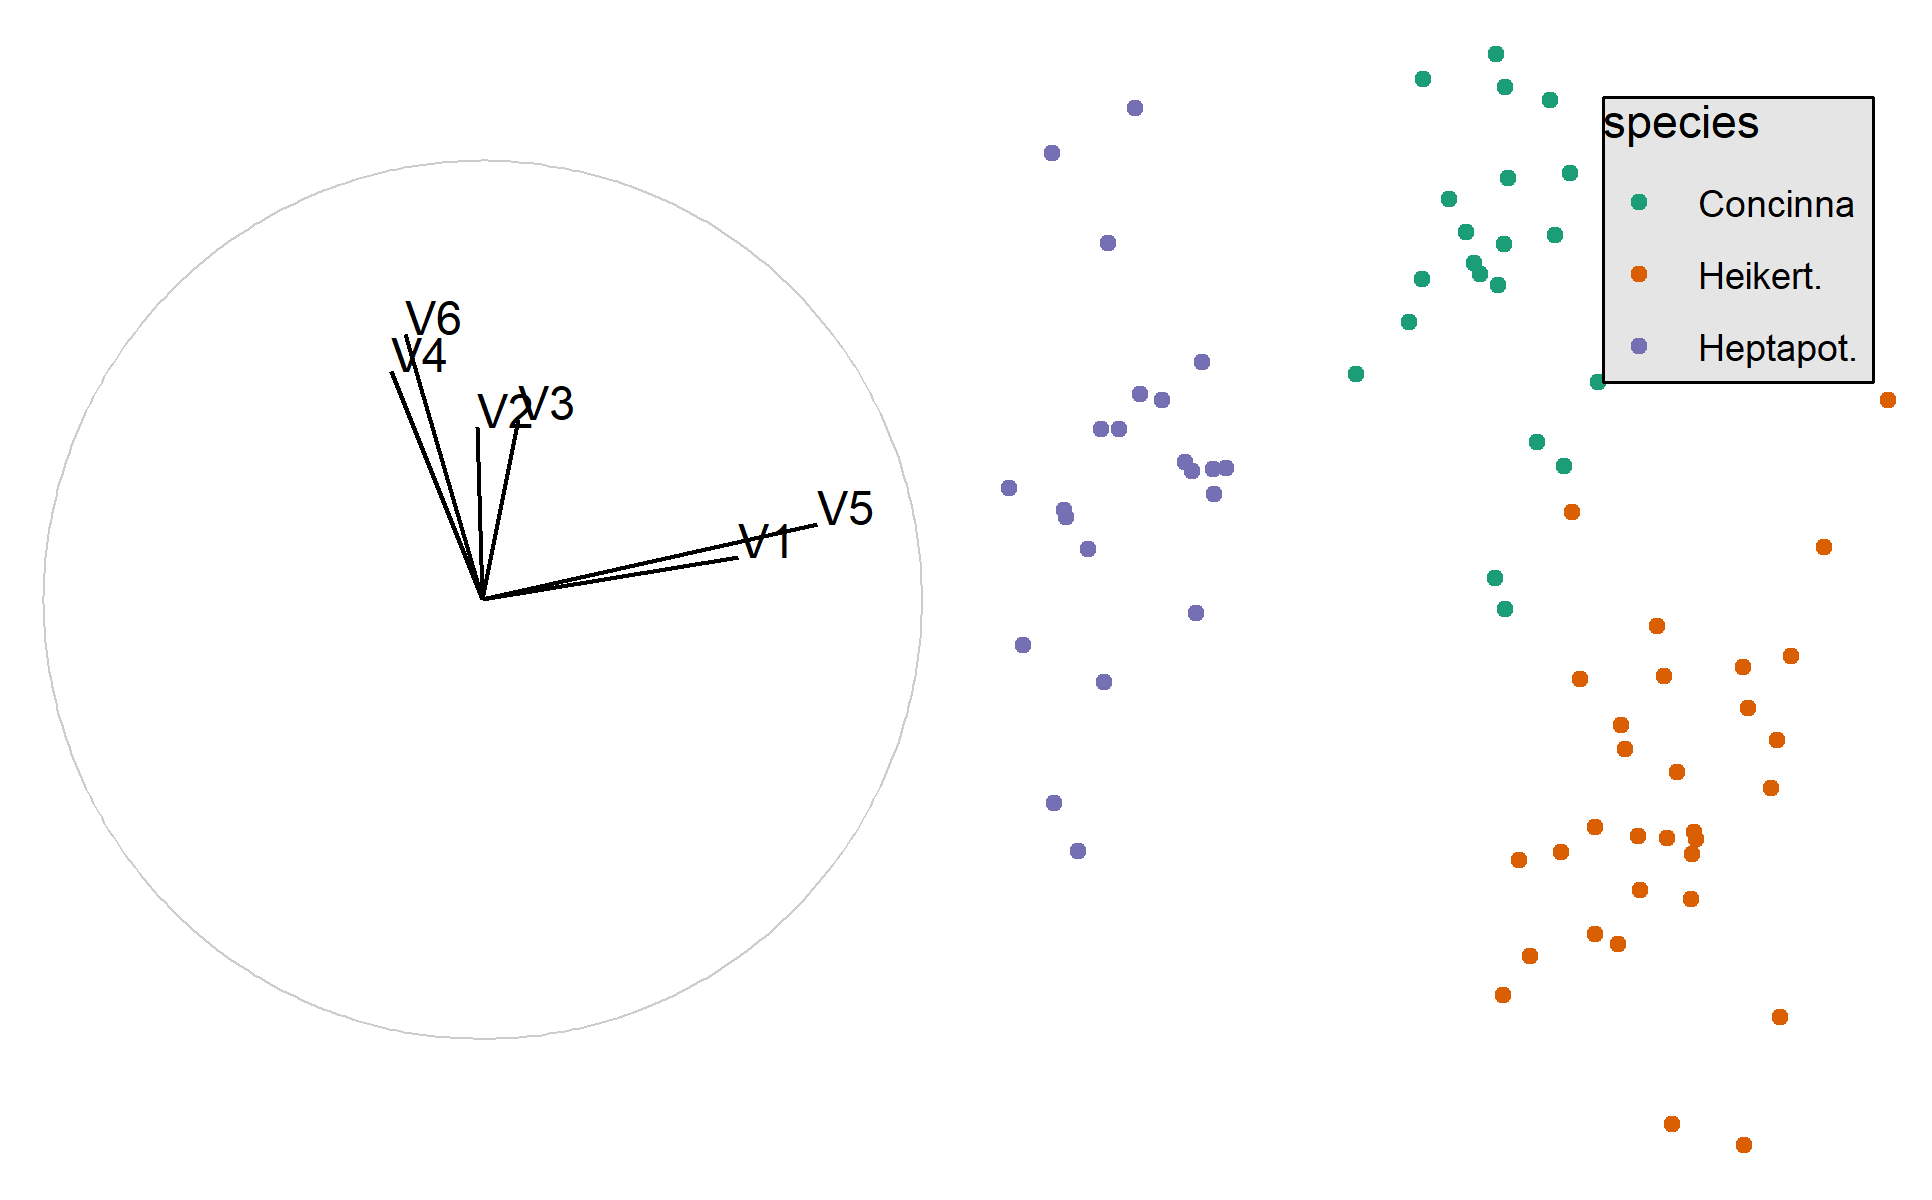
\includegraphics[width=6.71in]{./output/step0_basis+proj} \caption{basis and projection, holes guided tour of flea data}\label{fig:step0}
\end{figure}

Call the \texttt{view\_basis()} function to produce the left frame. In
touring typically we want dynamic display that looks through many such
views, however, you can project a single basis at any time through the
matrix multiplication
\(\textbf{X}_{[n,~p]} ~*~ \textbf{B}_{[p,~d]} ~=~ \textbf{P}_{d[n,~d]}\)
to reproduce the right frame.

\begin{Shaded}
\begin{Highlighting}[]
\NormalTok{view_basis <-}\StringTok{ }\ControlFlowTok{function}\NormalTok{(basis,}
                      \DataTypeTok{labels =} \KeywordTok{paste0}\NormalTok{(}\StringTok{"V"}\NormalTok{, }\DecValTok{1}\OperatorTok{:}\KeywordTok{nrow}\NormalTok{(basis))}
\NormalTok{) \{}
  \CommentTok{# Initialize}
\NormalTok{  p <-}\StringTok{ }\KeywordTok{nrow}\NormalTok{(basis)}
  \ControlFlowTok{if}\NormalTok{ (}\OperatorTok{!}\KeywordTok{is.data.frame}\NormalTok{(basis)) basis <-}\StringTok{ }\KeywordTok{as.data.frame}\NormalTok{(basis)}
\NormalTok{  ## circle}
\NormalTok{  angle <-}\StringTok{ }\KeywordTok{seq}\NormalTok{(}\DecValTok{0}\NormalTok{, }\DecValTok{2} \OperatorTok{*}\StringTok{ }\NormalTok{pi, }\DataTypeTok{length =} \DecValTok{360}\NormalTok{)}
\NormalTok{  circ  <-}\StringTok{ }\KeywordTok{data.frame}\NormalTok{(}\DataTypeTok{x =} \KeywordTok{cos}\NormalTok{(angle), }\DataTypeTok{y =} \KeywordTok{sin}\NormalTok{(angle))}
  
  \CommentTok{# graphics (reference frame)}
\NormalTok{  ## circle and set options}
\NormalTok{  gg1 <-}\StringTok{ }\NormalTok{ggplot2}\OperatorTok{::}\KeywordTok{ggplot}\NormalTok{() }\OperatorTok{+}\StringTok{ }\NormalTok{ggplot2}\OperatorTok{::}\KeywordTok{geom_path}\NormalTok{(}
    \DataTypeTok{data =}\NormalTok{ circ, }\DataTypeTok{color =} \StringTok{"grey80"}\NormalTok{, }\DataTypeTok{size =}\NormalTok{ .}\DecValTok{3}\NormalTok{, }\DataTypeTok{inherit.aes =}\NormalTok{ F,}
    \DataTypeTok{mapping =}\NormalTok{ ggplot2}\OperatorTok{::}\KeywordTok{aes}\NormalTok{(}\DataTypeTok{x =}\NormalTok{ circ}\OperatorTok{$}\NormalTok{x, }\DataTypeTok{y =}\NormalTok{ circ}\OperatorTok{$}\NormalTok{y)}
\NormalTok{  ) }\OperatorTok{+}
\StringTok{    }\NormalTok{ggplot2}\OperatorTok{::}\KeywordTok{scale_color_brewer}\NormalTok{(}\DataTypeTok{palette =} \StringTok{"Dark2"}\NormalTok{) }\OperatorTok{+}
\StringTok{    }\NormalTok{ggplot2}\OperatorTok{::}\KeywordTok{theme_void}\NormalTok{() }\OperatorTok{+}
\StringTok{    }\NormalTok{ggplot2}\OperatorTok{::}\KeywordTok{theme}\NormalTok{(}\DataTypeTok{legend.position =} \StringTok{"none"}\NormalTok{) }\OperatorTok{+}
\StringTok{    }\NormalTok{ggplot2}\OperatorTok{::}\KeywordTok{coord_fixed}\NormalTok{() }\CommentTok{# Do not use with plotly!}
\NormalTok{  ## Axes line segments}
\NormalTok{  gg2 <-}\StringTok{ }\NormalTok{gg1 }\OperatorTok{+}
\StringTok{    }\NormalTok{ggplot2}\OperatorTok{::}\KeywordTok{geom_segment}\NormalTok{(}
      \DataTypeTok{data =}\NormalTok{ basis, }
      \DataTypeTok{mapping =}\NormalTok{ ggplot2}\OperatorTok{::}\KeywordTok{aes}\NormalTok{(}\DataTypeTok{x =}\NormalTok{ basis[,}\DecValTok{1}\NormalTok{], }\DataTypeTok{y =}\NormalTok{ basis[,}\DecValTok{2}\NormalTok{], }\DataTypeTok{xend =} \DecValTok{0}\NormalTok{, }\DataTypeTok{yend =} \DecValTok{0}\NormalTok{)}
\NormalTok{    )}
\NormalTok{  ## Text labels}
\NormalTok{  gg3 <-}\StringTok{ }\NormalTok{gg2 }\OperatorTok{+}\StringTok{ }\NormalTok{ggplot2}\OperatorTok{::}\KeywordTok{geom_text}\NormalTok{(}
    \DataTypeTok{data =}\NormalTok{ basis, }\DataTypeTok{size =} \DecValTok{4}\NormalTok{, }\DataTypeTok{hjust =} \DecValTok{0}\NormalTok{, }\DataTypeTok{vjust =} \DecValTok{0}\NormalTok{, }\DataTypeTok{colour =} \StringTok{"black"}\NormalTok{,}
    \DataTypeTok{mapping =}\NormalTok{ ggplot2}\OperatorTok{::}\KeywordTok{aes}\NormalTok{(}\DataTypeTok{x =}\NormalTok{ basis[, }\DecValTok{1}\NormalTok{], }\DataTypeTok{y =}\NormalTok{ basis[, }\DecValTok{1}\NormalTok{], }\DataTypeTok{label =}\NormalTok{ labels)}
\NormalTok{  )}
  
\NormalTok{  gg3}
\NormalTok{\}}
\end{Highlighting}
\end{Shaded}

\subsection{Step 1 Choose variable of
interest}\label{step-1-choose-variable-of-interest}

Select a manipulation variable, \(k\). Initialize a zero vector \(e\),
and set the \(k\)-th element set to 1.

NOTE: Explanation has math, diagram and code

\begin{align*}
\textbf{e}_{k~[p,~1]} ~=~ 
  \begin{bmatrix}
    0 \\
    0 \\
    \vdots \\
    1 \\
    \vdots \\
    0
  \end{bmatrix}_{[p,~1]}
\end{align*}

In figure \ref{fig:step0}, above, notice the the variables 1 and 5 are
almost orthogonal to the other 4 variables and that V5 has a larger
contribution than V1. As such, let's select the 5-th variable as our
manipulation variable.

\subsection{Step 2 Create the manip
space}\label{step-2-create-the-manip-space}

NOTE: Explanation has math, diagram and code

Use the Gram-Schmidt process to orthonormalize the concatenation of the
basis and \(e\) yielding the manipulation space.

\begin{align*}
  \textbf{M}_{[p,~d+1]}
  &= Orthonormalize_{GS}( \textbf{B}_{[p,~d]}|\textbf{e}_{k~[p,~1]} ) \\
  &= Orthonormalize_{GS}
  \left(
    \begin{bmatrix}
      B_{1,~1} & \dots  & B_{1,~d} \\
      B_{2,~1} & \dots  & B_{2,~d} \\
      \vdots   & \ddots & \vdots   \\
      B_{k,~1} & \dots  & B_{k,~d} \\
      \vdots   & \ddots & \vdots   \\
      B_{p,~1} & \dots  & B_{p,~d}
    \end{bmatrix}
  ~|~
    \begin{bmatrix}
      0 \\
      0 \\
      \vdots \\
      1 \\
      \vdots \\
      0
    \end{bmatrix}
  \right)
\end{align*}

\begin{figure}
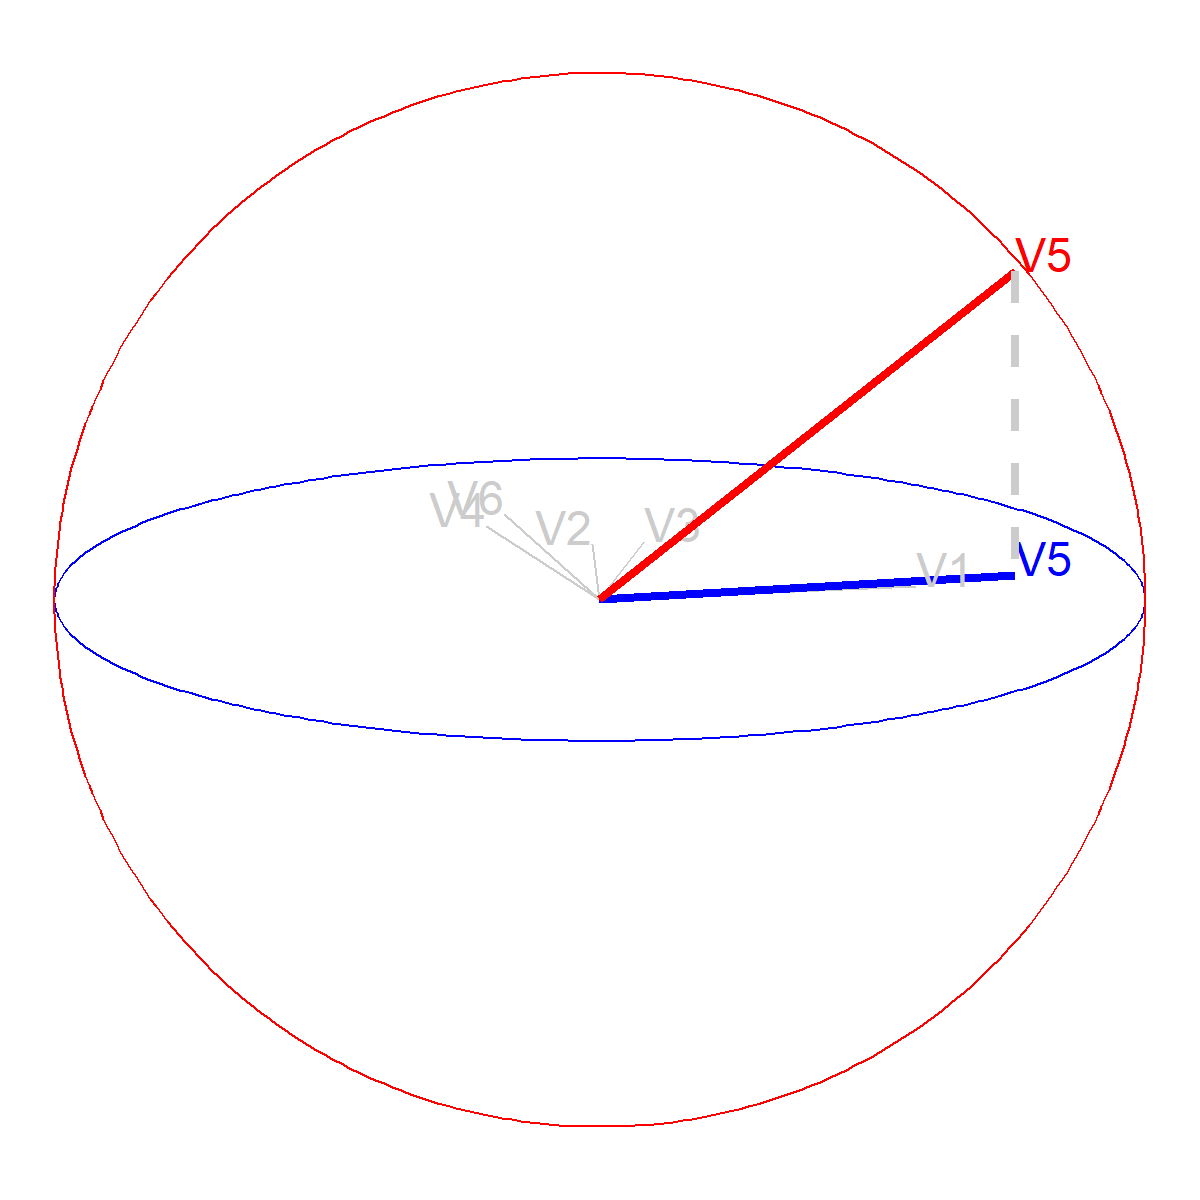
\includegraphics[width=16.67in]{./output/step2_manip_sp} \caption{manipulation space, holes guided tour of flea data}\label{fig:step2}
\end{figure}

\begin{Shaded}
\begin{Highlighting}[]
\NormalTok{view_manip_sp <-}\StringTok{ }\ControlFlowTok{function}\NormalTok{(basis,}
\NormalTok{                         manip_var,}
                         \DataTypeTok{manip_col =} \StringTok{"blue"}\NormalTok{,}
                         \DataTypeTok{theta =}\NormalTok{ pi }\OperatorTok{*}\StringTok{ }\DecValTok{5}\OperatorTok{/}\DecValTok{12}\NormalTok{,}
                         \DataTypeTok{z_col =} \StringTok{"red"}\NormalTok{,}
                         \DataTypeTok{labels =} \KeywordTok{paste0}\NormalTok{(}\StringTok{"V"}\NormalTok{, }\DecValTok{1}\OperatorTok{:}\KeywordTok{nrow}\NormalTok{(basis)) }
\NormalTok{) \{}
  \CommentTok{# Initialize}
  \ControlFlowTok{if}\NormalTok{ (}\OperatorTok{!}\KeywordTok{is.null}\NormalTok{(}\KeywordTok{colnames}\NormalTok{(basis))) labels <-}\StringTok{ }\KeywordTok{abbreviate}\NormalTok{(}\KeywordTok{colnames}\NormalTok{(basis), }\DecValTok{3}\NormalTok{)}
\NormalTok{  xyz <-}\StringTok{ }\ControlFlowTok{function}\NormalTok{(df) \{}\KeywordTok{colnames}\NormalTok{(df) <-}\StringTok{ }\KeywordTok{c}\NormalTok{(}\StringTok{"x"}\NormalTok{, }\StringTok{"y"}\NormalTok{, }\StringTok{"z"}\NormalTok{); df\}}
\NormalTok{  ## manip space}
\NormalTok{  m_sp <-}\StringTok{ }\KeywordTok{xyz}\NormalTok{(}\KeywordTok{data.frame}\NormalTok{(}\KeywordTok{create_manip_space}\NormalTok{(basis, manip_var)))}
\NormalTok{  p <-}\StringTok{ }\KeywordTok{nrow}\NormalTok{(m_sp)}
\NormalTok{  ## manip var asethetics}
\NormalTok{  col_v            <-}\StringTok{ }\KeywordTok{rep}\NormalTok{(}\StringTok{"grey80"}\NormalTok{, p)}
\NormalTok{  col_v[manip_var] <-}\StringTok{ }\NormalTok{manip_col}
\NormalTok{  siz_v            <-}\StringTok{ }\KeywordTok{rep}\NormalTok{(}\FloatTok{0.3}\NormalTok{, p)}
\NormalTok{  siz_v[manip_var] <-}\StringTok{ }\DecValTok{1}
\NormalTok{  ## circle}
\NormalTok{  angle <-}\StringTok{ }\KeywordTok{seq}\NormalTok{(}\DecValTok{0}\NormalTok{, }\DecValTok{2} \OperatorTok{*}\StringTok{ }\NormalTok{pi, }\DataTypeTok{length =} \DecValTok{360}\NormalTok{)}
\NormalTok{  circ  <-}\StringTok{ }\KeywordTok{data.frame}\NormalTok{(}\DataTypeTok{x =} \KeywordTok{cos}\NormalTok{(angle), }\DataTypeTok{y =} \KeywordTok{sin}\NormalTok{(angle), }\DataTypeTok{z =} \DecValTok{0}\NormalTok{)}
\NormalTok{  ## basis rotation}
\NormalTok{  rot   <-}\StringTok{ }\KeywordTok{matrix}\NormalTok{(}\KeywordTok{c}\NormalTok{(}\DecValTok{1}\NormalTok{,}\DecValTok{0}\NormalTok{,}\DecValTok{1}\NormalTok{, }\DecValTok{0}\NormalTok{,}\KeywordTok{cos}\NormalTok{(theta),}\KeywordTok{sinpi}\NormalTok{(theta)), }\CommentTok{# ,0,0,sin(theta))}
                  \DataTypeTok{ncol =} \DecValTok{3}\NormalTok{, }\DataTypeTok{byrow =}\NormalTok{ T)}
\NormalTok{  ## rotation spaces}
\NormalTok{  circ_r <-}\StringTok{ }\KeywordTok{xyz}\NormalTok{(}\KeywordTok{data.frame}\NormalTok{(}\KeywordTok{as.matrix}\NormalTok{(circ[, }\KeywordTok{c}\NormalTok{(}\DecValTok{1}\NormalTok{, }\DecValTok{2}\NormalTok{)]) }\OperatorTok\StringTok{ }\NormalTok{rot))}
\NormalTok{  m_sp_r <-}\StringTok{ }\KeywordTok{xyz}\NormalTok{(}\KeywordTok{data.frame}\NormalTok{(}\KeywordTok{as.matrix}\NormalTok{(m_sp[, }\KeywordTok{c}\NormalTok{(}\DecValTok{1}\NormalTok{, }\DecValTok{2}\NormalTok{)]) }\OperatorTok\StringTok{ }\NormalTok{rot))}
\NormalTok{  circ_z <-}\StringTok{ }\KeywordTok{data.frame}\NormalTok{(}\DataTypeTok{x =}\NormalTok{ circ}\OperatorTok{$}\NormalTok{x, }\DataTypeTok{y =}\NormalTok{ circ}\OperatorTok{$}\NormalTok{y }\OperatorTok{*}\StringTok{ }\KeywordTok{sin}\NormalTok{(theta))}
\NormalTok{  m_sp_z <-}\StringTok{ }\KeywordTok{data.frame}\NormalTok{(}\DataTypeTok{x =}\NormalTok{ m_sp[manip_var, }\StringTok{"x"}\NormalTok{],}
                       \DataTypeTok{y =}\NormalTok{ m_sp[manip_var, }\StringTok{"z"}\NormalTok{] }\OperatorTok{*}\StringTok{ }\KeywordTok{sin}\NormalTok{(theta))}
  
  \CommentTok{# Graphics (reference frame)}
\NormalTok{  ## xy circle and options}
\NormalTok{  gg1 <-}\StringTok{ }\NormalTok{ggplot2}\OperatorTok{::}\KeywordTok{ggplot}\NormalTok{() }\OperatorTok{+}\StringTok{ }\NormalTok{ggplot2}\OperatorTok{::}\KeywordTok{geom_path}\NormalTok{(}
    \DataTypeTok{data =}\NormalTok{ circ_r, }\DataTypeTok{color =}\NormalTok{ manip_col, }\DataTypeTok{size =}\NormalTok{ .}\DecValTok{3}\NormalTok{, }\DataTypeTok{inherit.aes =}\NormalTok{ F,}
    \DataTypeTok{mapping =}\NormalTok{ ggplot2}\OperatorTok{::}\KeywordTok{aes}\NormalTok{(}\DataTypeTok{x =}\NormalTok{ x, }\DataTypeTok{y =}\NormalTok{ y)}
\NormalTok{  ) }\OperatorTok{+}
\StringTok{    }\NormalTok{ggplot2}\OperatorTok{::}\KeywordTok{scale_color_brewer}\NormalTok{(}\DataTypeTok{palette =} \StringTok{"Dark2"}\NormalTok{) }\OperatorTok{+}
\StringTok{    }\NormalTok{ggplot2}\OperatorTok{::}\KeywordTok{theme_void}\NormalTok{() }\OperatorTok{+}
\StringTok{    }\NormalTok{ggplot2}\OperatorTok{::}\KeywordTok{theme}\NormalTok{(}\DataTypeTok{legend.position =} \StringTok{"none"}\NormalTok{) }\OperatorTok{+}
\StringTok{    }\NormalTok{ggplot2}\OperatorTok{::}\KeywordTok{coord_fixed}\NormalTok{() }\CommentTok{# Do not use with plotly!}
\NormalTok{  ## Axes line segments}
\NormalTok{  gg2 <-}\StringTok{ }\NormalTok{gg1 }\OperatorTok{+}
\StringTok{    }\NormalTok{ggplot2}\OperatorTok{::}\KeywordTok{geom_segment}\NormalTok{(}
      \DataTypeTok{data =}\NormalTok{ m_sp_r, }\DataTypeTok{size =}\NormalTok{ siz_v, }\DataTypeTok{colour =}\NormalTok{ col_v,}
      \DataTypeTok{mapping =}\NormalTok{ ggplot2}\OperatorTok{::}\KeywordTok{aes}\NormalTok{(}\DataTypeTok{x =}\NormalTok{ x, }\DataTypeTok{y =}\NormalTok{ y, }\DataTypeTok{xend =} \DecValTok{0}\NormalTok{, }\DataTypeTok{yend =} \DecValTok{0}\NormalTok{)}
\NormalTok{    )}
\NormalTok{  ## Text labels}
\NormalTok{  gg3 <-}\StringTok{ }\NormalTok{gg2 }\OperatorTok{+}\StringTok{ }\NormalTok{ggplot2}\OperatorTok{::}\KeywordTok{geom_text}\NormalTok{(}
    \DataTypeTok{data =}\NormalTok{ m_sp_r, }\DataTypeTok{size =} \DecValTok{4}\NormalTok{, }\DataTypeTok{colour =}\NormalTok{ col_v,}
    \DataTypeTok{vjust =} \StringTok{"outward"}\NormalTok{, }\DataTypeTok{hjust =} \StringTok{"outward"}\NormalTok{,}
    \DataTypeTok{mapping =}\NormalTok{ ggplot2}\OperatorTok{::}\KeywordTok{aes}\NormalTok{(}\DataTypeTok{x =}\NormalTok{ x, }\DataTypeTok{y =}\NormalTok{ y, }\DataTypeTok{label =}\NormalTok{ labels)}
\NormalTok{  )}
\NormalTok{  ## zx circle}
\NormalTok{  gg4 <-}\StringTok{ }\NormalTok{gg3 }\OperatorTok{+}\StringTok{ }\NormalTok{ggplot2}\OperatorTok{::}\KeywordTok{geom_path}\NormalTok{(}
    \DataTypeTok{data =}\NormalTok{ circ_z, }\DataTypeTok{color =}\NormalTok{ z_col, }\DataTypeTok{size =}\NormalTok{ .}\DecValTok{3}\NormalTok{, }\DataTypeTok{inherit.aes =}\NormalTok{ F,}
    \DataTypeTok{mapping =}\NormalTok{ ggplot2}\OperatorTok{::}\KeywordTok{aes}\NormalTok{(}\DataTypeTok{x =}\NormalTok{ x, }\DataTypeTok{y =}\NormalTok{ y)}
\NormalTok{  )}
\NormalTok{  ## z manip sp segments, projection line, label}
\NormalTok{  gg5 <-}\StringTok{ }\NormalTok{gg4 }\OperatorTok{+}\StringTok{ }\NormalTok{ggplot2}\OperatorTok{::}\KeywordTok{geom_segment}\NormalTok{(}
    \DataTypeTok{data =}\NormalTok{ m_sp_z, }\DataTypeTok{size =} \DecValTok{1}\NormalTok{, }\DataTypeTok{colour =}\NormalTok{ z_col,}
    \DataTypeTok{mapping =}\NormalTok{ ggplot2}\OperatorTok{::}\KeywordTok{aes}\NormalTok{(}\DataTypeTok{x =}\NormalTok{ x, }\DataTypeTok{y =}\NormalTok{ y, }\DataTypeTok{xend =} \DecValTok{0}\NormalTok{, }\DataTypeTok{yend =} \DecValTok{0}\NormalTok{)}
\NormalTok{  ) }\OperatorTok{+}\StringTok{ }\NormalTok{ggplot2}\OperatorTok{::}\KeywordTok{geom_segment}\NormalTok{(}
    \DataTypeTok{data =}\NormalTok{ m_sp_z, }\DataTypeTok{size =} \DecValTok{1}\NormalTok{, }\DataTypeTok{colour =} \StringTok{"grey80"}\NormalTok{, }\DataTypeTok{linetype =} \DecValTok{2}\NormalTok{,}
    \DataTypeTok{mapping =}\NormalTok{ ggplot2}\OperatorTok{::}\KeywordTok{aes}\NormalTok{(}\DataTypeTok{x =}\NormalTok{ x, }\DataTypeTok{y =}\NormalTok{ y, }\DataTypeTok{xend =}\NormalTok{ x, }\DataTypeTok{yend =}\NormalTok{ m_sp_r[manip_var, }\StringTok{"y"}\NormalTok{] )}
\NormalTok{  ) }\OperatorTok{+}\StringTok{ }\NormalTok{ggplot2}\OperatorTok{::}\KeywordTok{geom_text}\NormalTok{(}
    \DataTypeTok{data =}\NormalTok{ m_sp_z, }\DataTypeTok{size =} \DecValTok{4}\NormalTok{, }\DataTypeTok{colour =}\NormalTok{ z_col,}
    \DataTypeTok{vjust =} \StringTok{"outward"}\NormalTok{, }\DataTypeTok{hjust =} \StringTok{"outward"}\NormalTok{,}
    \DataTypeTok{mapping =}\NormalTok{ ggplot2}\OperatorTok{::}\KeywordTok{aes}\NormalTok{(}\DataTypeTok{x =}\NormalTok{ x, }\DataTypeTok{y =}\NormalTok{ y, }\DataTypeTok{label =}\NormalTok{ labels[manip_var])}
\NormalTok{  )}
  
\NormalTok{  gg5}
\NormalTok{\}}
\end{Highlighting}
\end{Shaded}

\subsection{Step 3 Generate rotation}\label{step-3-generate-rotation}

NOTE: Explanation has math, diagram and code

Select a vector \(\phi_i\), the angle of out-of plane rotation,
orthogonal to the projection plane (relative to \(\phi_1\), the
transformation \(\phi_i\) - \(\phi_1\) proved to be helpful to discuss
\(\phi\) relative to the Z axis).

\textbf{For } \(i\) \textbf{in 1 to n\_slides:}

For each \(\phi_i\), post multiply the manipulation space by a rotation
matrix, producing as many basis-projections.

\begin{align*}
  \textbf{P}_{b[p,~d+1,~i]}
  &= \textbf{M}_{[p,~d+1]} ~*~ \textbf{R}_{[d+1,~d+1]} 
    ~~~~~~~~~~~~~~~~~~~\text{For the $d=2$ case:} \\
  &= \begin{bmatrix}
    M_{1,~1} & M_{1,~2} & M_{1,~3} \\
    M_{2,~1} & M_{2,~2} & M_{2,~3} \\
    \vdots   & \vdots   & \vdots   \\
    M_{p,~1} & M_{p,~2} & M_{p,~3}
  \end{bmatrix}_{[p,~d+1]}
    ~*~
  \begin{bmatrix}
    c_\theta^2 c_\phi s_\theta^2 &
    -c_\theta s_\theta (1 - c_\phi) &
    -c_\theta s_\phi \\
    -c_\theta s_\theta (1 - c_\phi) &
    s_\theta^2 c_\phi + c_\theta^2 &
    -s_\theta s_\phi \\
    c_\theta s_\phi &
    s_\theta s_\phi &
    c_\phi
  \end{bmatrix}_{[3,~3]}
\end{align*}

Where:

\begin{description}
  \item[$\theta$] is the angle that lies on the projection plane ($ie.$ on the XY plane)
  \item[$\phi$] is the angle orthogonal to the projection plane ($ie.$ in the Z direction)
  \item[$c_\theta$] is the cosine of $\theta$
  \item[$c_\phi$]   is the cosine of $\phi$
  \item[$s_\theta$] is the sine of   $\theta$
  \item[$s_\phi$]   is the sine of   $\phi$
\end{description}

To get back to data-space post multiply each projection basis by the
data, for the data projection.

\begin{align}
  \textbf{P}_{d[n,~d+1]}
    &= \textbf{X}_{[n,~p]} ~*~ \textbf{P}_{b[p,~d+1]} \\
    &= \begin{bmatrix}
      X_{1,~1} & \dots & X_{1,~p} \\
      X_{2,~1} & \dots & X_{2,~p} \\
      \vdots   & \vdots & \vdots  \\
      X_{n,~1} & \dots & X_{n,~p}
    \end{bmatrix}_{[n,~p]}
      ~*~
    \begin{bmatrix}
      P_{b:1,~1} & P_{b:1,~2} & P_{b:1,~3} \\
      P_{b:2,~1} & P_{b:2,~2} & P_{b:2,~3} \\
      \vdots     & \vdots     & \vdots     \\
      P_{b:p,~1} & P_{b:p,~2} & P_{b:p,~3}
    \end{bmatrix}_{b[p,~d+1]}
\end{align}

\begin{figure}
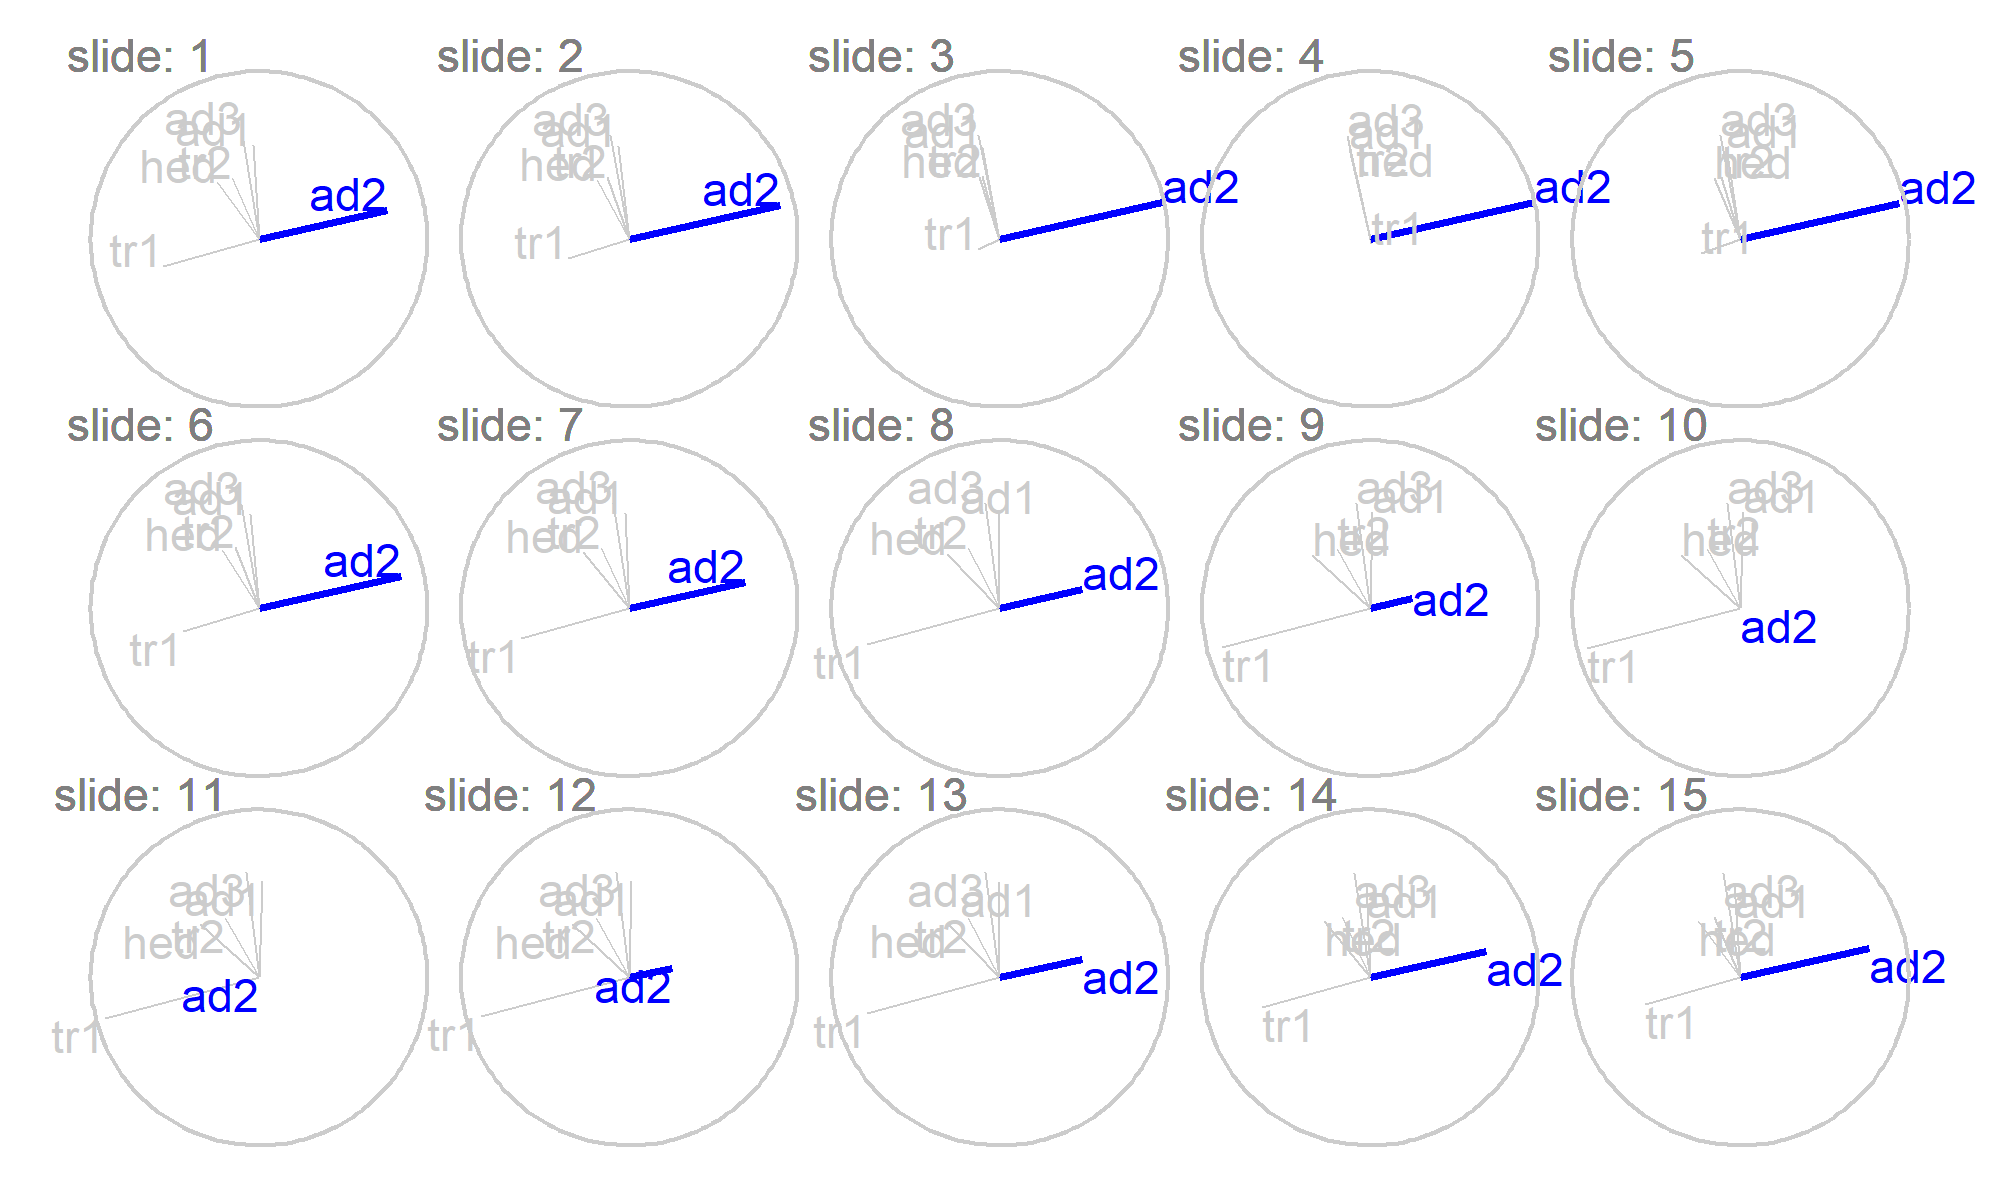
\includegraphics[width=27.78in]{./output/step3_manual_tour} \caption{manual tour, holes guided tour of flea data}\label{fig:step3}
\end{figure}

\begin{Shaded}
\begin{Highlighting}[]
\NormalTok{manual_tour <-}\StringTok{ }\ControlFlowTok{function}\NormalTok{(}\DataTypeTok{basis =} \OtherTok{NULL}\NormalTok{,}
\NormalTok{                        manip_var,  }\CommentTok{# column number}
                        \DataTypeTok{theta =} \OtherTok{NULL}\NormalTok{,      }\CommentTok{# (radians)}
                        \DataTypeTok{phi_min =} \DecValTok{0}\NormalTok{,       }\CommentTok{# (radians)}
                        \DataTypeTok{phi_max =}\NormalTok{ .}\DecValTok{5} \OperatorTok{*}\StringTok{ }\NormalTok{pi, }\CommentTok{# (radians)}
                        \DataTypeTok{n_slides =} \DecValTok{20}
\NormalTok{) \{}
  \CommentTok{# Initalize}
  \ControlFlowTok{if}\NormalTok{ (}\OperatorTok{!}\KeywordTok{is.matrix}\NormalTok{(basis)) basis <-}\StringTok{ }\KeywordTok{as.matrix}\NormalTok{(basis)}
  \ControlFlowTok{if}\NormalTok{ (}\KeywordTok{is.null}\NormalTok{(theta)) theta <-}\StringTok{ }\KeywordTok{atan}\NormalTok{(basis[manip_var, }\DecValTok{2}\NormalTok{] }\OperatorTok{/}\StringTok{ }\NormalTok{basis[manip_var, }\DecValTok{1}\NormalTok{])}
\NormalTok{  manip_space    <-}\StringTok{ }\KeywordTok{create_manip_space}\NormalTok{(}\DataTypeTok{basis =}\NormalTok{ basis, }\DataTypeTok{manip_var =}\NormalTok{ manip_var)}
\NormalTok{  p              <-}\StringTok{ }\KeywordTok{nrow}\NormalTok{(basis)}
\NormalTok{  d              <-}\StringTok{ }\KeywordTok{ncol}\NormalTok{(basis)}
\NormalTok{  phi_start      <-}\StringTok{ }\KeywordTok{acos}\NormalTok{(}\KeywordTok{sqrt}\NormalTok{(basis[manip_var, }\DecValTok{1}\NormalTok{]}\OperatorTok{^}\DecValTok{2} \OperatorTok{+}\StringTok{ }\NormalTok{basis[manip_var, }\DecValTok{2}\NormalTok{]}\OperatorTok{^}\DecValTok{2}\NormalTok{))}
\NormalTok{  phi_start_sign <-}\StringTok{ }\NormalTok{phi_start }\OperatorTok{*}\StringTok{ }\KeywordTok{sign}\NormalTok{(manip_space[manip_var, }\DecValTok{1}\NormalTok{])}
\NormalTok{  phi_inc        <-}\StringTok{ }\DecValTok{2} \OperatorTok{*}\StringTok{ }\KeywordTok{abs}\NormalTok{(phi_max }\OperatorTok{-}\StringTok{ }\NormalTok{phi_min) }\OperatorTok{/}\StringTok{ }\NormalTok{(n_slides }\OperatorTok{-}\StringTok{ }\DecValTok{3}\NormalTok{)}
  \KeywordTok{stopifnot}\NormalTok{(phi_min }\OperatorTok{<=}\StringTok{ }\NormalTok{phi_start }\OperatorTok{&}\StringTok{ }\NormalTok{phi_max }\OperatorTok{>=}\StringTok{ }\NormalTok{phi_start)}
  
\NormalTok{  interpolate_walk <-}\StringTok{ }\ControlFlowTok{function}\NormalTok{(seq_start, seq_end)\{}
    \CommentTok{# Initialize for interpolate_slides()}
\NormalTok{    slide        <-}\StringTok{ }\DecValTok{0}
\NormalTok{    new_slide    <-}\StringTok{ }\OtherTok{NULL}
\NormalTok{    seq_start    <-}\StringTok{ }\NormalTok{seq_start }\OperatorTok{+}\StringTok{ }\NormalTok{phi_start_sign }\CommentTok{# Transform such that phi is relative to Z=0, rather than phi_start}
\NormalTok{    seq_end      <-}\StringTok{ }\NormalTok{seq_end   }\OperatorTok{+}\StringTok{ }\NormalTok{phi_start_sign}
\NormalTok{    phi_inc_sign <-}\StringTok{ }\NormalTok{phi_inc }\OperatorTok{*}\StringTok{ }\KeywordTok{ifelse}\NormalTok{(seq_end }\OperatorTok{>}\StringTok{ }\NormalTok{seq_start, }\DecValTok{1}\NormalTok{, }\OperatorTok{-}\DecValTok{1}\NormalTok{) }
\NormalTok{    phi_len      <-}\StringTok{ }\KeywordTok{length}\NormalTok{(}\KeywordTok{seq}\NormalTok{(seq_start, seq_end, phi_inc_sign))}
\NormalTok{    interp       <-}\StringTok{ }\KeywordTok{array}\NormalTok{(}\DataTypeTok{dim =} \KeywordTok{c}\NormalTok{(p, d, phi_len))}
    
    \CommentTok{# Create slide, store in interpolation}
    \ControlFlowTok{for}\NormalTok{ (phi }\ControlFlowTok{in} \KeywordTok{seq}\NormalTok{(seq_start, seq_end, phi_inc_sign)) \{}
\NormalTok{      slide <-}\StringTok{ }\NormalTok{slide }\OperatorTok{+}\StringTok{ }\DecValTok{1}
\NormalTok{      interp[,, slide] <-}\StringTok{ }\KeywordTok{rotate_manip_space}\NormalTok{(manip_space, theta, phi)[, }\DecValTok{1}\OperatorTok{:}\DecValTok{2}\NormalTok{]}
\NormalTok{    \}}
    \KeywordTok{return}\NormalTok{(interp)}
\NormalTok{  \}}
  
\NormalTok{  walk1 <-}\StringTok{ }\KeywordTok{interpolate_walk}\NormalTok{(phi_start, phi_min)}
\NormalTok{  walk2 <-}\StringTok{ }\KeywordTok{interpolate_walk}\NormalTok{(phi_min, phi_max)}
\NormalTok{  walk3 <-}\StringTok{ }\KeywordTok{interpolate_walk}\NormalTok{(phi_max, phi_start)}
\NormalTok{  walk4 <-}\StringTok{ }\KeywordTok{interpolate_walk}\NormalTok{(phi_start, phi_start)}
  
\NormalTok{  m_tour <-}\StringTok{ }\KeywordTok{array}\NormalTok{(}\KeywordTok{c}\NormalTok{(walk1, walk2, walk3, walk4), }\DataTypeTok{dim =} \KeywordTok{c}\NormalTok{(p, d, n_slides))}
  \KeywordTok{attr}\NormalTok{(m_tour, }\StringTok{"manip_var"}\NormalTok{) <-}\StringTok{ }\NormalTok{manip_var}
  
  \KeywordTok{return}\NormalTok{(m_tour)}
\NormalTok{\}}
\end{Highlighting}
\end{Shaded}

\section{Display projection sequence}\label{display-projection-sequence}

Plot the first 2 variables from each projection in sequence for an XY
scatterplot. The remaining variable is sometimes linked to a data point
aesthetic to produce depth cues used in conjunction with the XY
scatterplot.

\section{Installation}\label{installation}

spinifex is open source and hosted on
\href{https://github.com/nspyrison/spinifex}{GitHub}. The development
version is available for download by running
\texttt{devtools::install\_github("nspyrison/spinifex")} on your R
console.

\section{Application}\label{application}

apply manual tours to Ursula fig 1 here: NOTE: Examples from
\url{https://arxiv.org/abs/1806.09742}

First stab at reproducing Fig8 from the PDFSense paper, is hosted here:
\href{https://nspyrison.netlify.com/else/pdfsense_fig8repex/}{nspyrison.netlify.com}

\section{Source}\label{source}

The code used to generate this chapter can be found at this
\href{https://github.com/nspyrison/Confirmation/blob/master/03-spinifex.Rmd}{GitHub
page}.

\section{Discussion}\label{discussion}

Future work:

\begin{itemize}
\tightlist
\item
  other rotation mechanisms like Givens and Householder
\item
  oblique should be defined.
\item
  other display types, would work for 1D displays, but others would need
  redefinition difference dimensions
\item
  shiny app, for choosing manip variable, providing different starting
  projections
\end{itemize}

\chapter{Display dimensionality}\label{ch:disp_dim}

\begin{itemize}
\tightlist
\item
  XGobbi vs the C2
\end{itemize}

\chapter{Human-computer interaction of 3d
projections}\label{ch:hci_3dproj}

\begin{itemize}
\tightlist
\item
  Tour in 3D
\item
  ImAxes / IATK
\end{itemize}

\appendix

\chapter{Additional stuff}\label{additional-stuff}

You might put some computer output here, or maybe additional tables.

Note that line 5 must appear before your first appendix. But other
appendices can just start like any other chapter.

\printbibliography[heading=bibintoc]



\end{document}
